
%(BEGIN_QUESTION)
% Copyright 2006, Tony R. Kuphaldt, released under the Creative Commons Attribution License (v 1.0)
% This means you may do almost anything with this work of mine, so long as you give me proper credit

Modern pH and temperature (thermocouple) transmitters are constructed with extremely high input impedances (typically in the hundreds of megaohms).  Explain why a high input impedance voltmeter is important when measuring the voltage output by a source, when the voltage in question is very small.

\vskip 10pt

In the days before the advent of solid-state digital multimeters with their operational amplifier (high impedance) inputs, a technique called {\it null-balance} was used to accurately measure small voltages such as those produced by thermocouple junctions and pH probes.  This ``potentiometric'' technique allowed people to use rather primitive voltmeter technology without incurring the errors that would be experienced if the voltmeter were directly connected to the signal source.

Examine the circuits shown below, and explain how the two meters (one ``galvanometer'' and one voltmeter) plus a power source and a potentiometer would be used to measure voltage from the signal source (pH probe or thermocouple junction):

$$\includegraphics[width=15.5cm]{i00621x01.eps}$$

\underbar{file i00621}
%(END_QUESTION)





%(BEGIN_ANSWER)

The problem may be summarized using just one word: {\it loading}.  All voltmeters draw some current from the signal under test, but analog-style voltmeters drew signficantly more current than their modern DMM equivalents.  This is a problem because the current drawn by a voltmeter tends to ``load down'' the voltage output by the signal source, resulting in a negative error (reading less voltage than the source is actually trying to output).

\vskip 10pt

The ``null-balance'' technique works like this:

\begin{itemize}
\item{} Adjust the potentiometer until the sensitive galvanometer registers {\it zero current}
\item{} Read the voltmeter's indication -- this will be precisely equal to the signal source
\end{itemize}

Galvanometers are nothing more than hyper-sensitive ammeters.  When the galvanometer reads zero, you know the potentiometer's output voltage is precisely equal to the signal source voltage.  This is why the voltmeter's reading in this condition is precisely equal to the signal source voltage.  However, the current required by the voltmeter to allow it to function is being supplied by the battery, not by the signal source.  This ``unloads'' the signal source so that it does not have to power the voltmeter.

%(END_ANSWER)





%(BEGIN_NOTES)


%INDEX% Measurement, analytical: pH

%(END_NOTES)


